\chapter{BoBshield API}
\label{kap:3}


\section{API pre Simulink}
\label{kap:3.2}

Simulink je grafické programovacie prostredie založené na MATLABe a určené pre modelovanie, simuláciu a analýzu dynamických systémov.  Jeho hlavným rozhraním je nástrojom pre vytváranie grafických blokových diagramov a sada blokových knižníc, určených pre rôzne typy aplikácií. Ide o nástroj často využívaní pri automatickom riadení a využíva sa aj pri digitálnom spracovaní signálov. Táto časť práce sa venuje API vytvorenému v tomto prostredí a určenému pre riadenie nášho zariadenia. 

\subsection{Knižnica}
\label{kap:3.2.1}
Pre tvorbu rozhrania pre programovanie nášho zariadenie v prostredí Simulink je potrebné vytvoriť vlastnú knižnicu, ktoré obsahuje potrebné funkcie pre komunikáciu so zariadením. Táto sa ale svojou formou líši od knižnice vytvorenej pre prostredie Arduino IDE. V porovnaní s ňou neobsahuje kód ako taký ale skladá sa s jednotlivých blokov, ktorých úlohou je zastrešiť určitú funkciu a následným spájaním blokov do diagramu vytvárame výsledný program, ktorý je následne pri kompilácii nahraný do mikropočítača. Knižnica je teda klasický súbor pre Simulink model ( .slx ) obsahujúci dané bloky a do zoznamu knižníc v programovacom prostredí je pridaný prostredníctvo MATLAB kódu. Aby sme knižnicu vedeli dostúpiť je potrebné spustiť súbor s názvom InstallMatlabAndSimulink nachádzajúci sa v knižnici AutomationShield. Jeho úlohou je nastaviť všetky cesty tak aby program vedel nájsť potrebné súbory pre implementáciu knižnice. 

Jednotlivé bloky nachádzajúce sa v BOBShield knižnici teda slúžia rovnako ako funkcie naprogramované v knižnici pre Arduino IDE a zastrešujú rovnaké úlohy.

Prvým blokom je Actuator Write, ktorého úlohou je riadenie servomotora. Spracúva vstupnú hodnotu vchádzajúcu do bloku a následne nastavuje uhol otočenia servomotora v rozsahu, ktorý sme preň určili. Pri nastavovaní parametrov bloku si môžeme zvoliť typ vstupu, vchádzajúceho do bloku a to z 2 možností – v percentách a vo vzdialenosti reprezentovanej v mm.  Dôležitým parametrom je taktiež rozsah uhlov, ktorý pre blok nastavíme. Môžeme buď nechať defaultne prednastavené hodnoty v rozsahu -30\degree až +30\degree alebo zvoliť možnosť manuálneho nastavenia vlastného rozsahu kde si zvolíme minimálny a maximálny uhol otočenia.

\begin{figure}
	\centering
	\includegraphics[width=50mm]{obr/servo.png}
	\caption{blok Actuator Write}\label{OBRAZOK 3.1.1} 
\end{figure} 

Blok Reference Read nám v diagrame reprezentuje potenciometer umiestnený na BOBShielde. Slúži na získavanie hodnôt z potenciometra, ktorý môže byť využitý ako referenčná hodnota pri riadení systému. Po kliknutí pravým tlačidlom myši na daný blok v schéme si môže užívateľ nastaviť spôsob akým budú hodnoty z potenciometra prezentované v Simulinku. Je možné zvoliť si z 3 možností, ktoré môžeme vidieť v sekcii Readout type. Prvou je získanie hodnoty v percentách, kde hodnoty, ktoré získavame, budú z intervalu od 0 po 100 v závislosti od polohy bežca potenciometra. Ďalšou možnosťou je získavanie hodnôt v podobe napätia v rozsahu od 0 po 5 V. Poslednou dostupnou možnosťou nastavenia čítania hodnôt z potenciometra je analógová hodnota z intervalu od 0 po 1023.  V závislosti od potreby užívateľa blok poskytuje teda určitú flexibilitu v závislosti od aplikácie v ktorej ho chceme využiť.

\begin{figure}
	\centering
	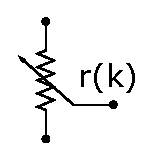
\includegraphics[width=30mm]{obr/Potentiometer.eps}
	\caption{blok Reference Read}\label{OBRAZOK 3.1.2} 
\end{figure} 

Ďalším blokom je Sensor Read a slúži nám na získavanie aktuálnej polohy guličky v trubičke. Ide o blok slúžiaci na komunikáciu mikropočítača s naším ToF snímačom VL6180X prostredníctvom I2C protokolu. Používateľ si môže vybrať z typov výstupných hodnôt zo snímača. Prvou možnosťou je vzdialenosť v mm, ktorá nám dáva vzdialenosť guličky od snímača v trubičke. Ďalšou z možnosti je pozícia guličky v mm. Ide o úpravu vzdialenosti, kde sa za počiatočnú pozíciu považuje koncový bod trubičky v ktorom sa nenachádza ToF snímač, teda výstupné hodnoty sú inverzné voči vzdialenosti. Pri voľbe výstupu v percentách sú potrebné kalibračné hodnoty aby vedel blok učiť minimálnu a maximálnu meranú hodnotu pre daný typ telesa v trubičke. Tie je možné zadať nižšie v okne parametrov bloku kedy si môžeme zvoliť buď defaultne nastavené hodnoty – 0 až 100 mm alebo nastaviť nami namerané krajné hodnoty pomocou manuálneho zadávania.

\begin{figure}
	\centering
	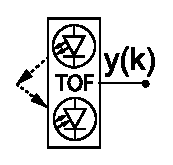
\includegraphics[width=30mm]{obr/SensorRead.eps}
	\caption{blok Sensor Read}\label{OBRAZOK 3.1.3} 
\end{figure} 

Posledným blokom je blok Filtration slúži na vyhľadenie šumu snímača....


\subsection{Príklady}
\label{kap:3.2.2}

\section{API pre Arduino IDE}
\label{kap:3.3}

\subsection{Filtrácia}
\label{kap:3.3.1}

Pri meraniach presnosti ToF snímača pre rôzne materiály, povrchy a farby guličiek sme mohli pozorovať šum, ktorý nám pri nameraných hodnotách vznikal. Hoci tento nežiaduci jav nie je možné celkom odstrániť, môžeme jeho dopad na namerané hodnoty výrazne znížiť pomocou implementácie jednoduchej filtrácie nameraných hodnôt vhodnou metódou.
Pre našu aplikáciu sme testovali 3 typy filtrácia a to pomocou aritmetického priemeru, aritmetického plávajúceho a váženého plávavjúceho priemeru. Pri testovaní sme postupovali nasledovne. Základom bolo získanie súboru nameraných hodnôt, na ktorý budeme môcť aplikovať filtre a následne navzájom porovnať ich výstupy. Vstup je pre všetky typy filtrov identický a preto môžeme spoľahlivejšie rozhodnúť o tom, ktorý z filtrov si zvolíme. Tieto hodnoty vstupu sme získali meraním polohy guličky pri jej posune z jednej koncovej polohy trubičky k druhej, pri minimálnom naklonení trubičky. Hodnoty boli získané a merané ešte na pôvodnej verzii zariadenia – BOBShield R2. 

Pri aritmetickom priemere sme z určitého počtu nameraných hodnôt urobili aritmetický priemer a výstupom bola 1 hodnota, z čoho vyplýva, že frekvencia, s ktorou sme merali je násobne väčšia ako frekvencia, získavania filtrovaných hodnôt. To môže mať za následok spomalenie systému z hľadiska rýchlosti reakcie na zmenu polohy guličky. Vlastnosti daného typu filtráciu vieme ovplyvniť počtom nameraných hodnôt, z ktorých robíme aritmetický priemer. Zvyšovanie počtu hodnôt má za následok väčšie vyhladenie výslednej krivky, no zároveň spôsobuje určité oneskorenie, čo môže byť pozorované hlavne keď gulička rýchlo mení svoju polohu. 

Rozdiel pri plávajúcom aritmetickom priemere je ten, že je založený na princípe zberu a ukladaní určitého počtu hodnôt, pričom pri každom ďalšom meraní sa nám najstaršia hodnota vymaže a pozíciu prvej hodnoty zaujme najnovšie nameraná hodnota. Z tohto súboru hodnôt sa nám pri každom meraní vypočíta aritmetický priemer, teda frekvencia merania a frekvencia získavania nameraných hodnôt je identická.

Vážený plávajúci priemer je založený na princípe je založený na rovnakom princípe práce s nameranými hodnotami ako plávajúci aritmetický priemer. Rozdielom je, že každá hodnota má inú váhu (ako vyplýva z názvu), teda má rozdielny vplyv na výslednú hodnotu.  Výsledná hodnota sa následne vypočíta podľa nasledujúceho vzorca:



\begin{align}
	\label{rovnica.3.3.1.1}
	priemer =\frac{\sum_{i=1}^{N}x_i*p(x_i)}{\sum_{i=1}^{N}p(x_i)} = \frac{ x_1*p(x_1)+x_2p(x_2)+\cdots +x_N*p(x_N)}{ p(x_1)+p(x_2)+\cdots +p(x_N)}
\end{align}

Vlastnosti filtrácie teda vieme ovplyvňovať jednak počtom hodnôt, z ktorých vážený priemer robíme, ale aj zmenou parametrov ovplyvňujúcich váhu jednotlivých hodnôt, teda vplyv na výsledok.

Vzorku hodnôt, na ktorej sme porovnávali vplyv jednotlivých typov filtrov sme si vykreslili do grafu v prostredí MATLAB spolu s grafmi hodnôt získaných po aplikácii filtrov. Následne sme menili parametre filtrov, či už išlo o počet hodnôt, z ktorých sme tvorili priemer alebo pri váženom priemere, o nastavenie parametrov váženia.

Pri procese hľadania parametrov pre vážený priemer sme uvažovali faktor zabúdania. Ide o bezrozmerné číslo z intervalu 0 až 1 a od jeho výberu závisí aké budú parametre jednotlivých váh pre dané hodnoty. Ak si zvolíme faktor zabúdania 0.9, väčšiu váhu budú mať práve staršie dáta. Naopak ak si zvolíme číslo blížiace sa k 0, dôraz bude kladený na najnovšie hodnoty. Jednotlivé koeficienty váh sa na základe faktora zabúdania získajú zo vzorca  \ref{rovnica.3.3.1.2}, kde $\lambda$ predstavuje faktor zabúdania. Pre rýchle systémy je lepšou voľbou výber menších hodnôt faktora.

\begin{align}
	\label{rovnica.3.3.1.2}
	p_{n+1} = p_n*\lambda+1
\end{align}


Na obrázku \ref{OBRAZOK 3.3.1.1} môžeme vidieť graf filtrácie pomocou aritmetického priemeru pre rozdielny počet hodnôt, z ktorých sme priemer získali.  Hoci vyhladenie krivky vyzerá veľmi dobre, oproti plávajúcemu priemeru, hodnoty získavame s oveľa nižšou frekvenciou, čo vytvára oneskorenie reakcie na rýchlu zmenu polohy guličky. Preto je určite vhodnejšou variantov jeden z typov plávajúcich priemerov.

\begin{figure}
	\centering
	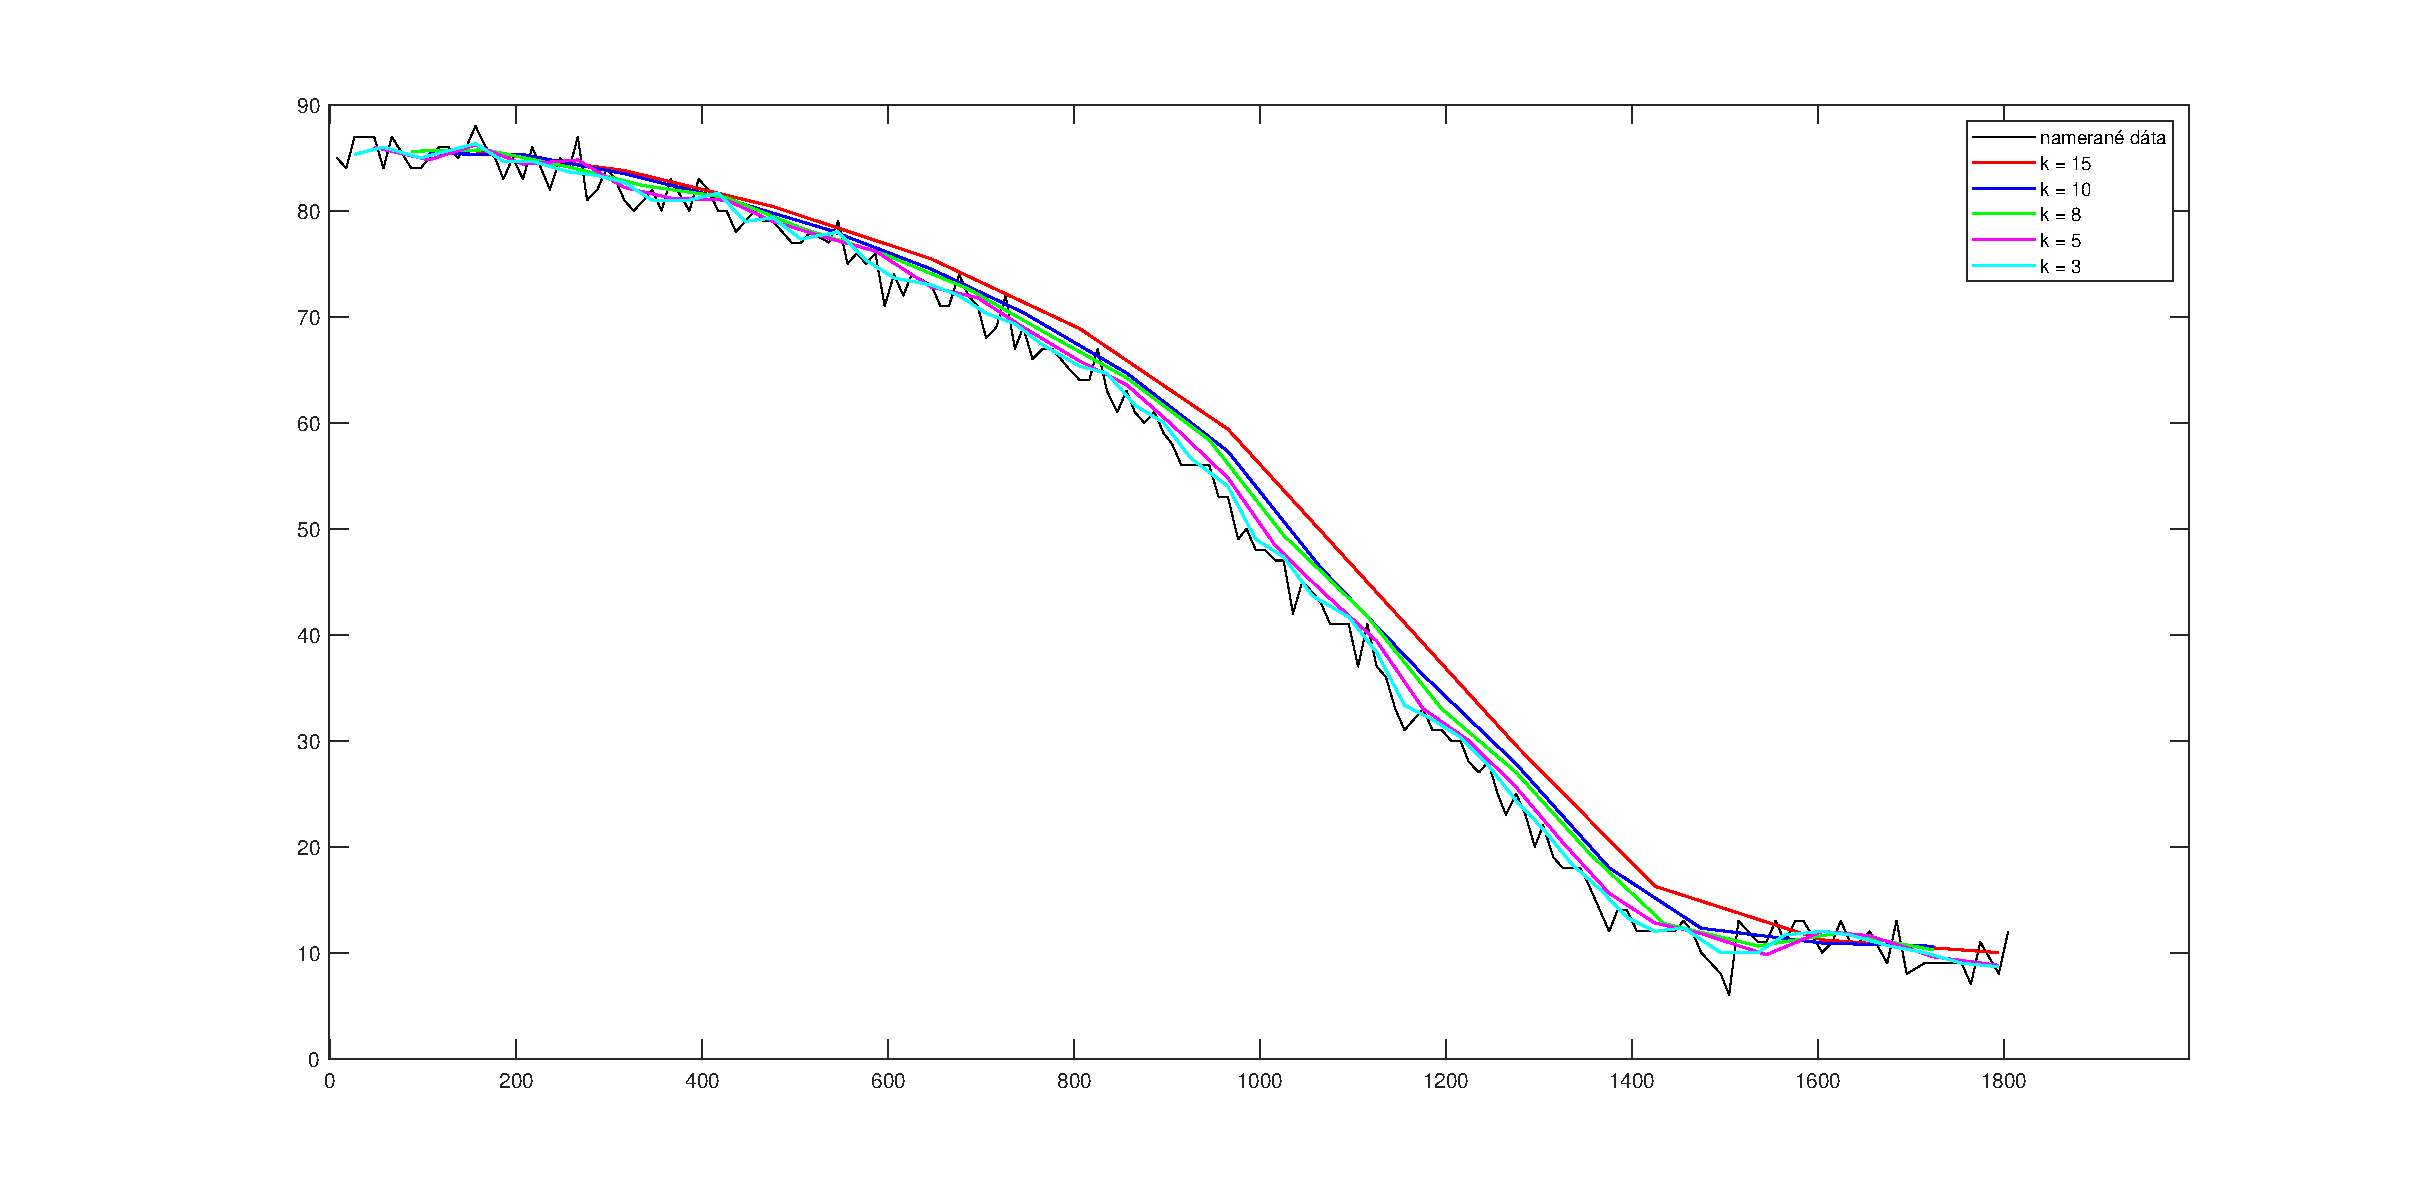
\includegraphics[width=170mm]{obr/aritmeticky.eps}
	\caption{Aritmetický priemer}\label{OBRAZOK 3.3.1.1} 
\end{figure}

Na ďalšom grafe (obr. \ref{OBRAZOK 3.3.1.2} ) môžeme vidieť filtráciu prostredníctvom plávajúceho aritmetického priemeru. Rovnako sme testovali rôzne počty hodnôt z ktorých sme daný priemer robili. Z grafu môžeme vidieť, že pri vyšších počtoch hodnôt sa krivka výrazne lepšie vyhladí, no zároveň je na grafe očividné oneskorenie oproti nefiltrovaným dátam. Z daných možností, ktoré sme testovali sme sa rozhodli pre filtráciu pomocou 5 posledných hodnôt. Krivka dobre kopíruje nefiltrované dáta z hľadiska oneskorenia a zároveň dosahuje prijateľné vyhladenie šumu.

\begin{figure}
	\centering
	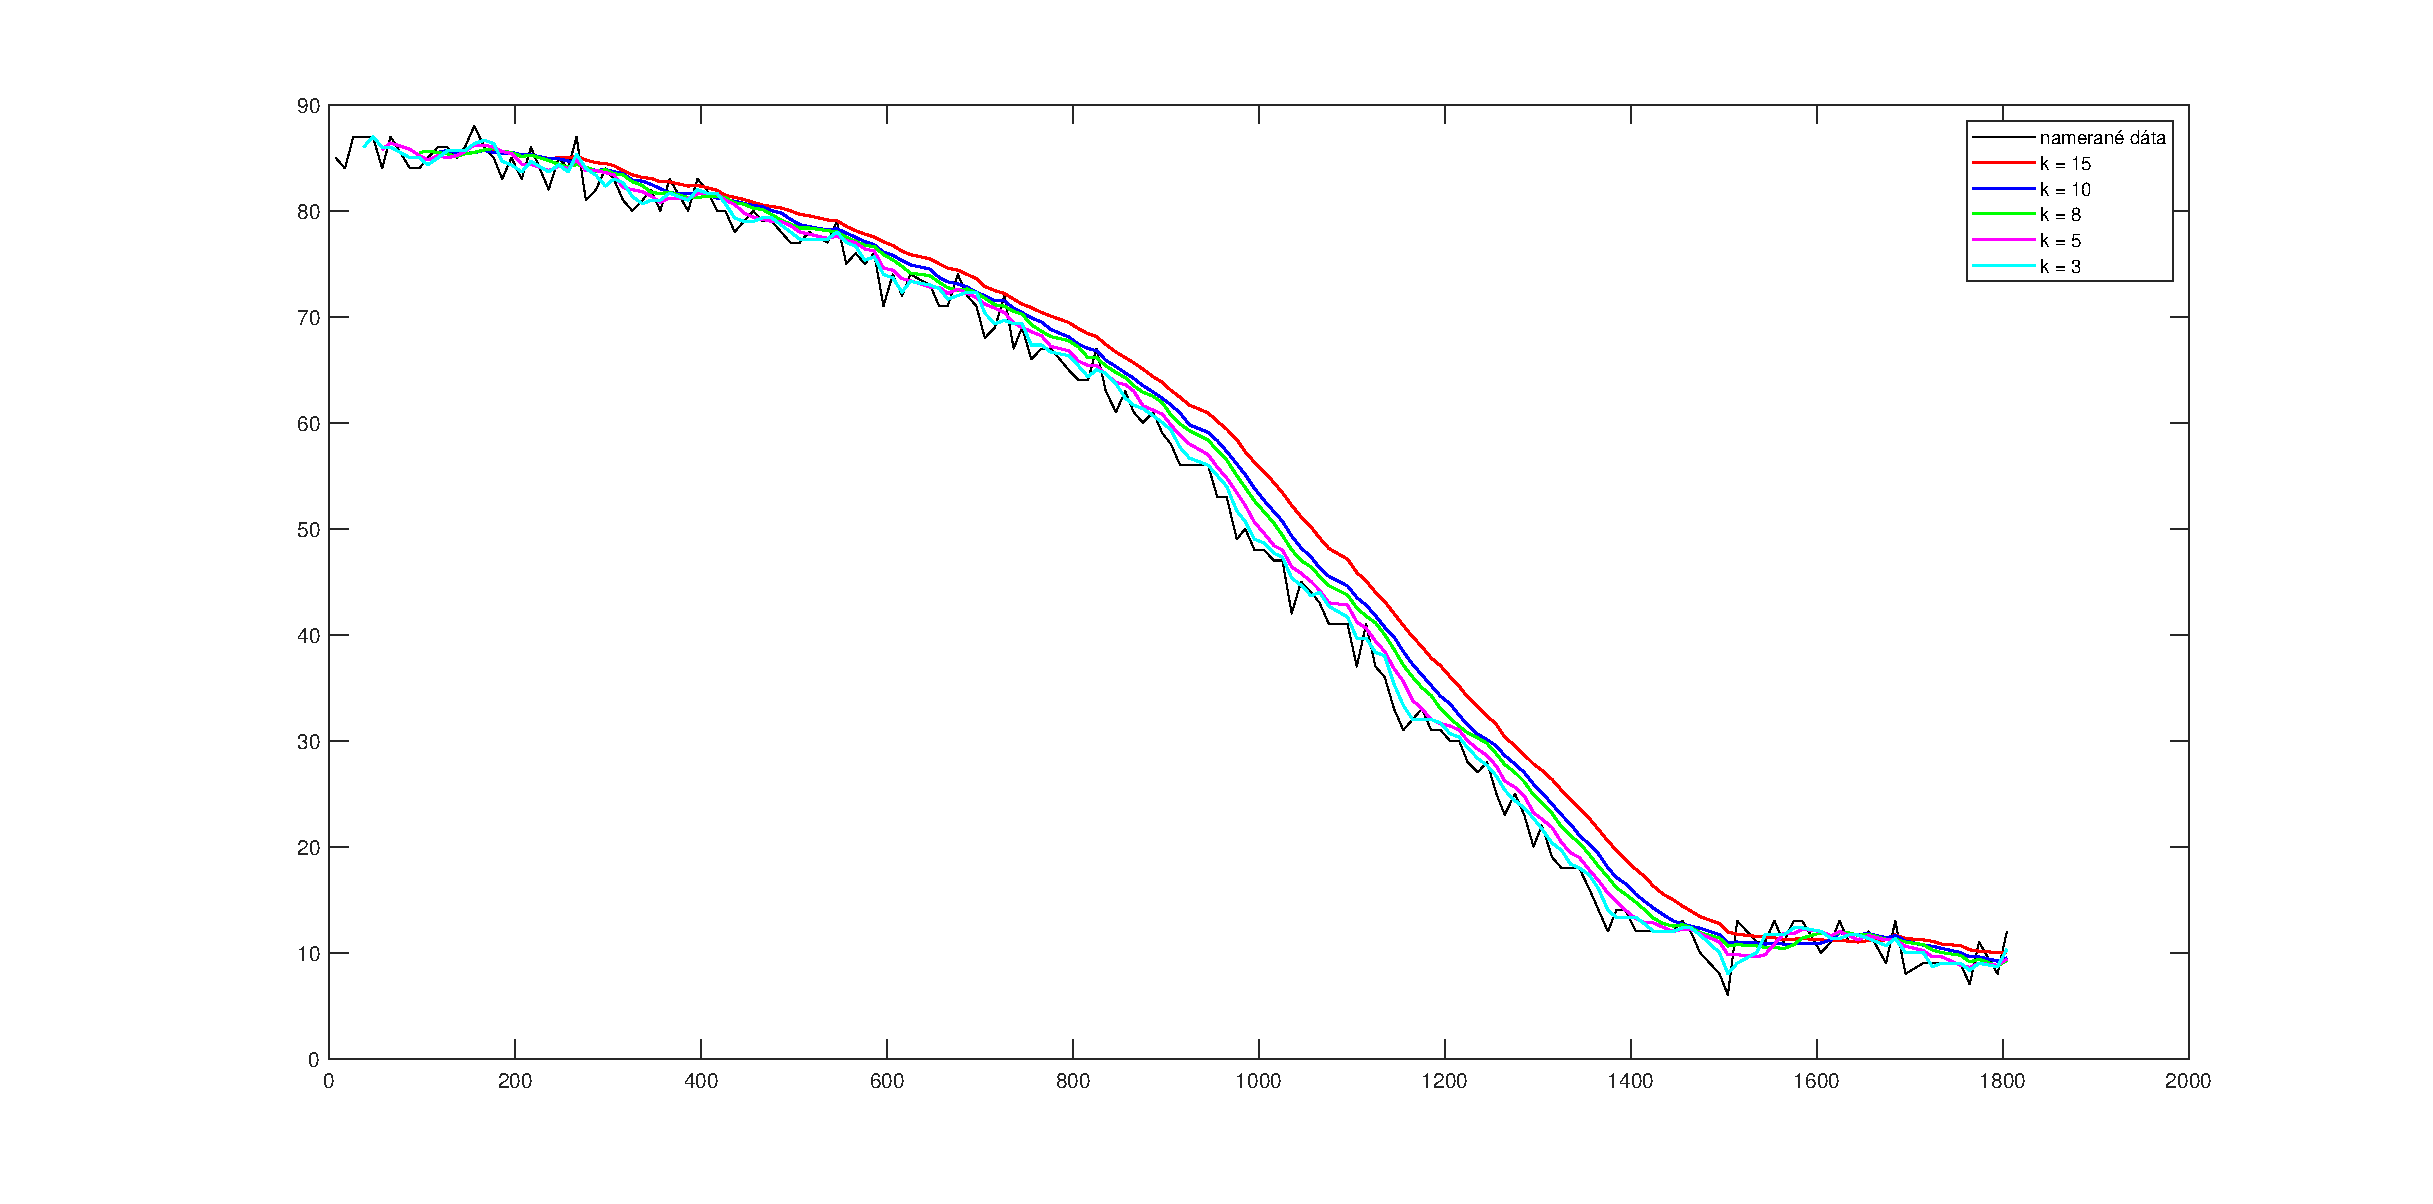
\includegraphics[width=170mm]{obr/plavajuciAritmeticky.eps}
	\caption{Plávajúci aritmetický priemer}\label{OBRAZOK 3.3.1.2} 
\end{figure}

Na grafe (obr. \ref{OBRAZOK 3.3.1.3} ) vidíme porovnanie filtrácie pomocou plávajúceho váženého priemeru z 5 hodnôt pre rozdielne faktory zabúdania. Môžeme vidieť, že rozdiel medzi jednotlivými krivkami je minimálny. Rozhodli sme sa zvoliť faktor zabúdania $\lambda = 0.4$ , keďže potrebujeme rýchlu reakciu na zmenu aktuálnej vzdialenosti, čiže dôraz na posledné hodnoty.

\begin{figure}
	\centering
	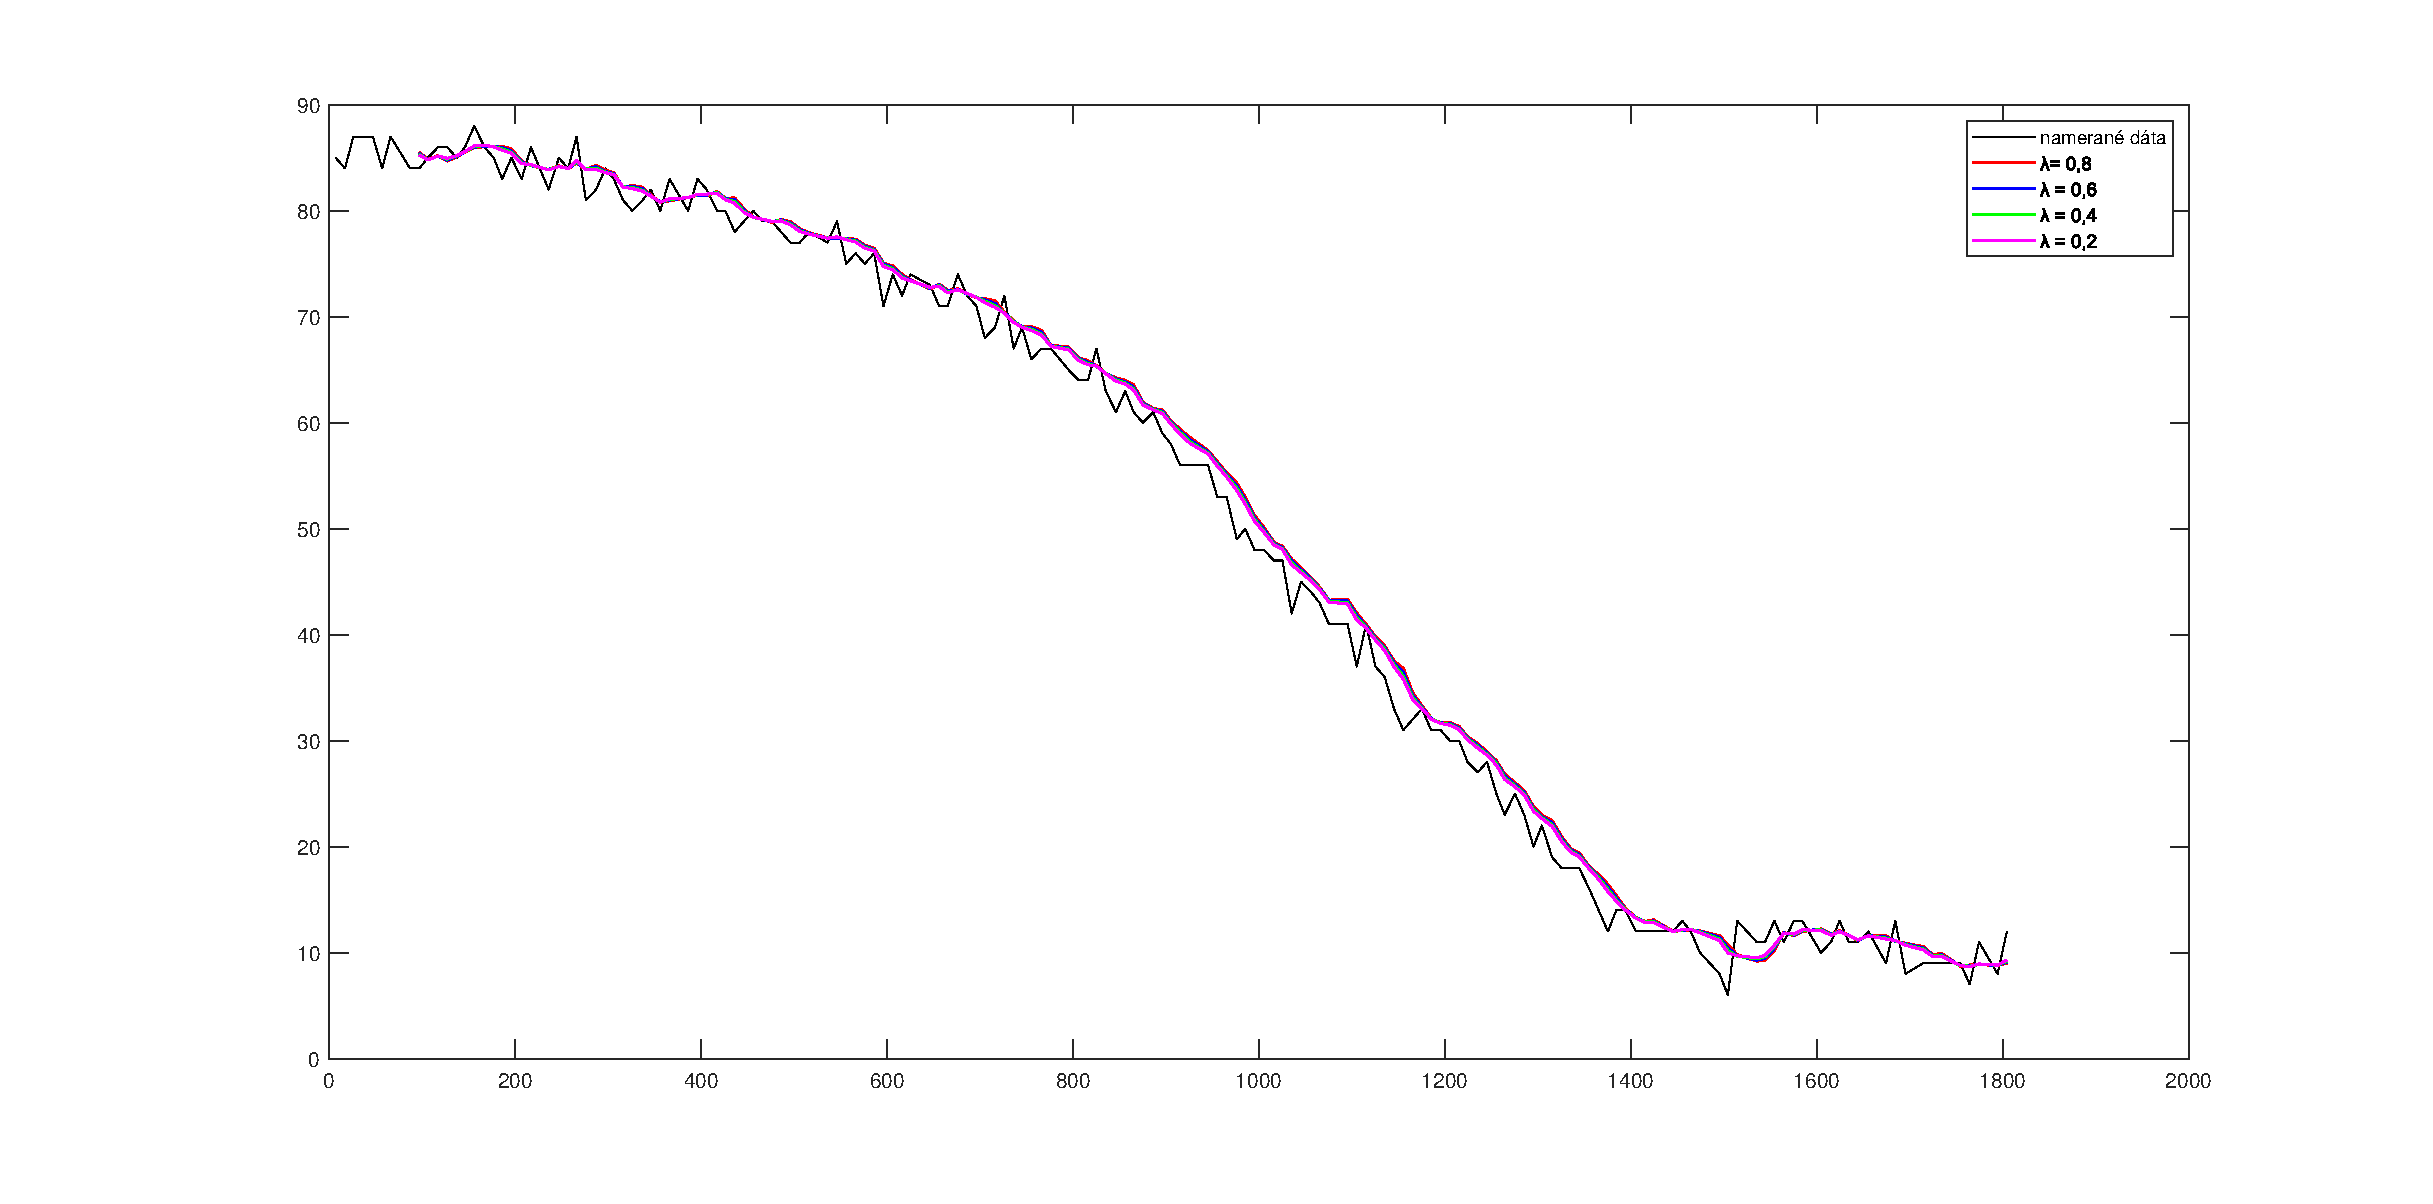
\includegraphics[width=170mm]{obr/plavajuciVazeny.eps}
	\caption{Plávajúci vážený priemer}\label{OBRAZOK 3.3.1.3} 
\end{figure}


Na obrázku \ref{OBRAZOK 3.3.1.4} môžeme vidieť porovnanie filtrácie plávajúceho aritmetického a váženého priemeru spolu s pôvodnými, nefiltrovanými nameranými hodnotami. Môžeme vidieť, že rozdiel medzi krivkami je minimálny. Jednoduchšou voľbou z hľadiska výpočtov je určite aritmetický priemer, čím budeme šetriť pamäť mikropočítača a výsledok bude takmer identický. Z tohto dôvodu sme sa rozhodli pre filtráciu pomocou plávajúceho aritmetického priemeru, počítaného z 5 posledných nameraných hodnôt.  

\begin{figure}
	\centering
	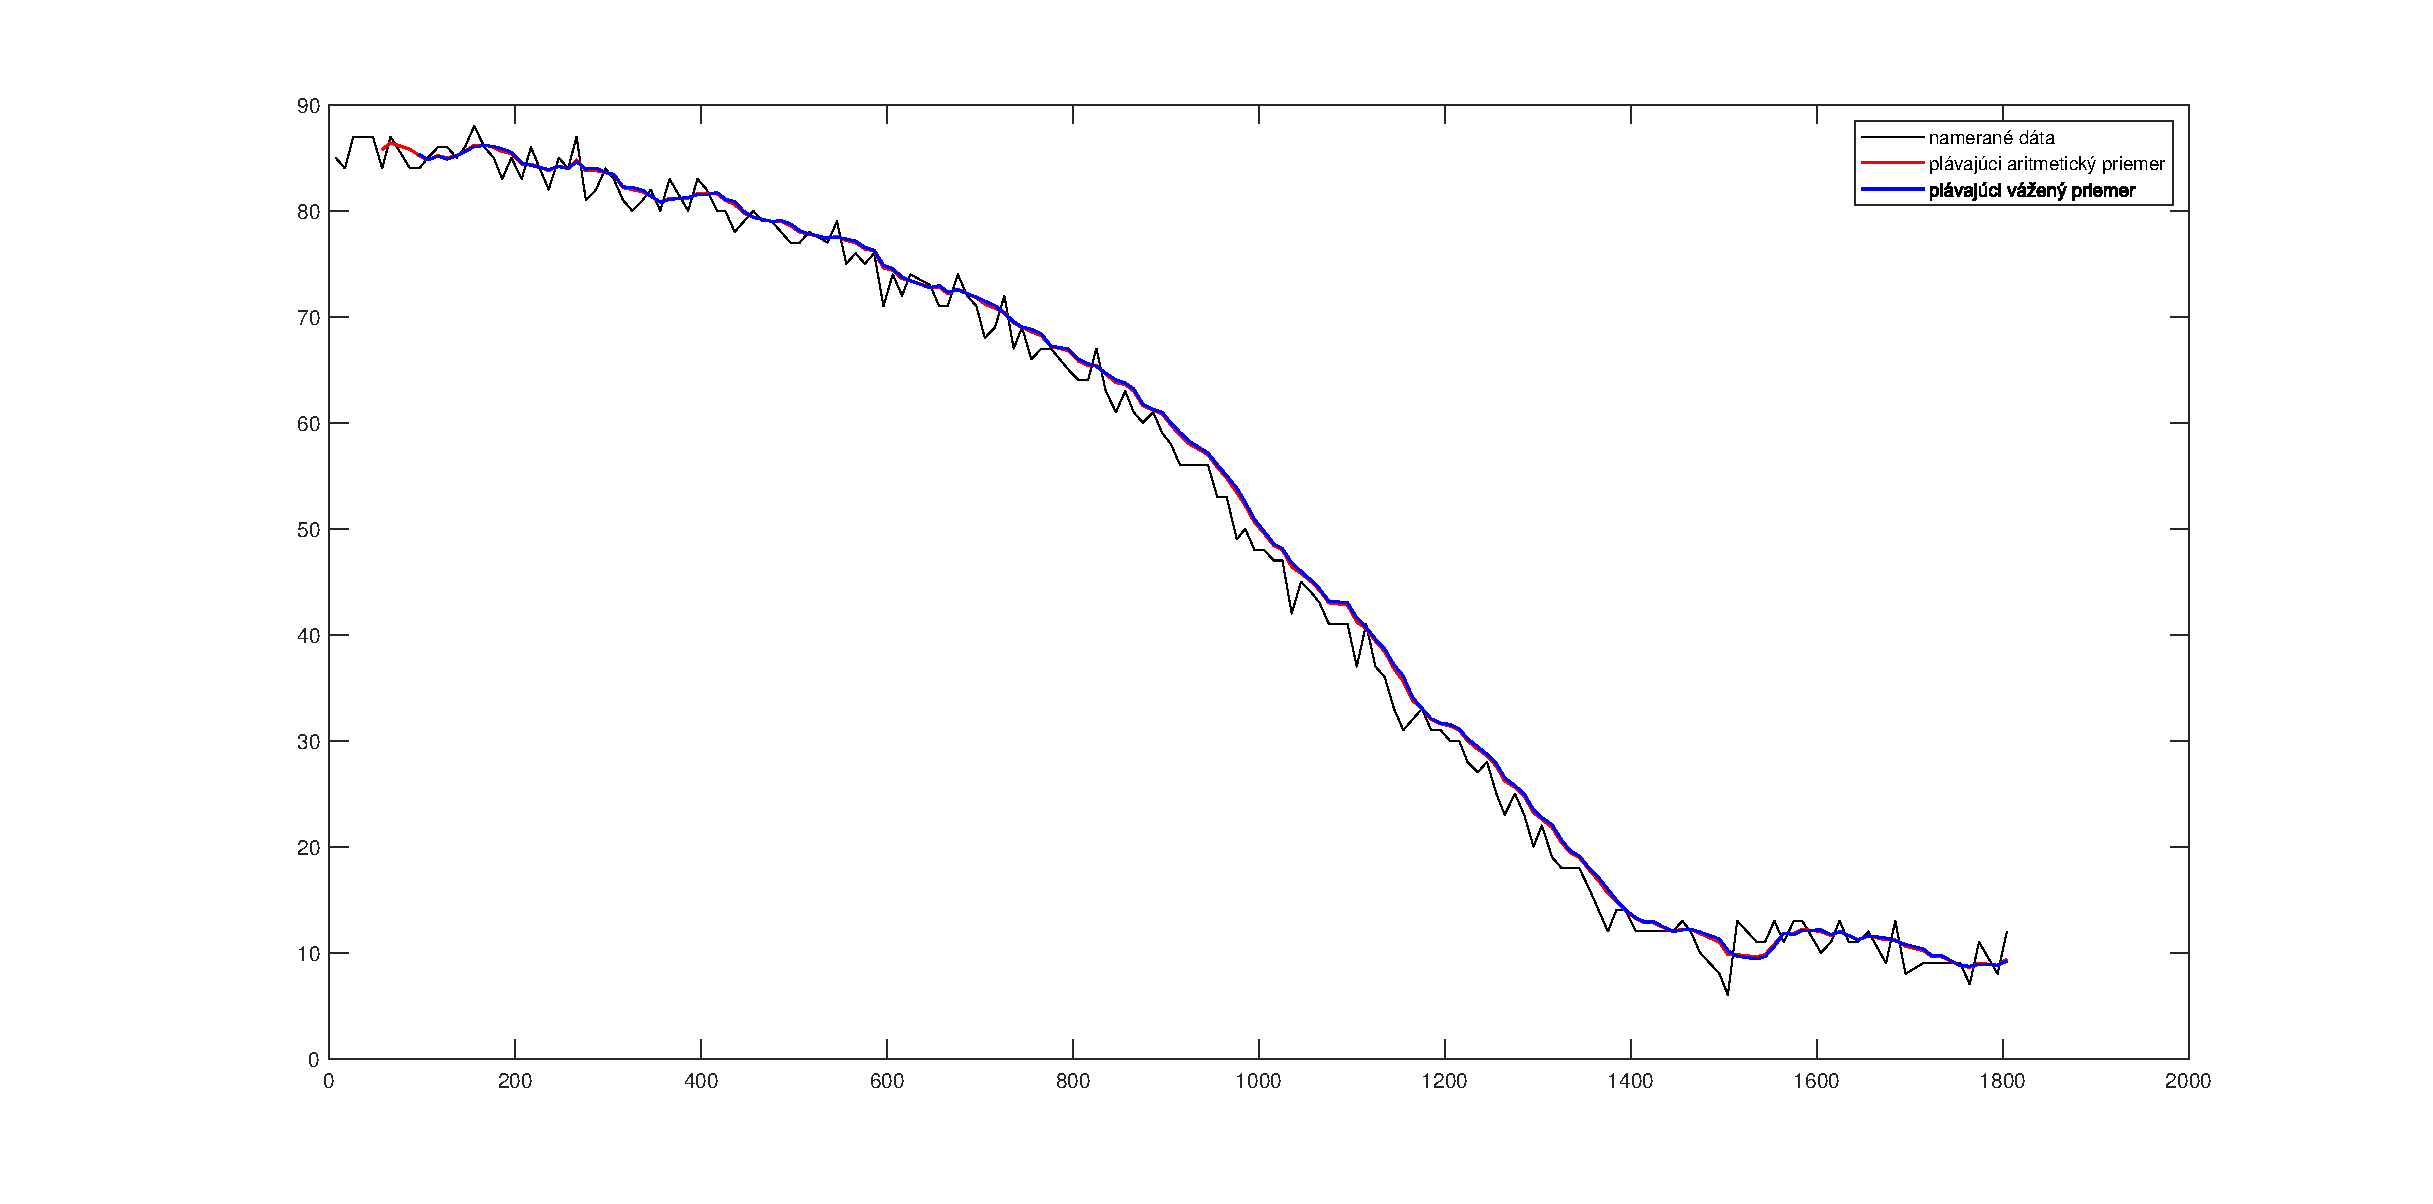
\includegraphics[width=170mm]{obr/aritmetickyVSvazeny.eps}
	\caption{Porovnanie plávajúceho artimetického a váženeého priemeru}\label{OBRAZOK 3.3.1.4} 
\end{figure}
